
\begin{frame}{Talk Outline}
  \begin{enumerate}
  \item Background: Core Model and Implementation
    \air
  \item Work 1: Rethinking Model Training (\textit{Beam Search Optimization})
    \air

  \item \textbf{Work 2:} Rethinking  Generation  (\textit{Learning Neural Templates})
    \air

  \item Future Directions
  \end{enumerate}
\end{frame}




% \begin{frame}{Part 4: Deep Latent-Variable Mdoels}

%    \begin{center}
%   \begin{tikzpicture}
%     \node[rounded corners, thick, draw] (ana) at (-15mm, 15mm) {Analysis};
%     \node[rounded corners, thick, fill=yellow,  draw] (meth) at (0mm, 30mm) {\ Methods\phantom{p}};
%     \node[rounded corners, thick, draw] (app) at (25mm, 30mm) {Applications};
%     \node[rounded corners, thick, fill=yellow, draw] (und) at (35mm, 15mm) {Understanding};
%     \node[rounded corners, thick, draw] (dep) at (25mm, 0mm){Scaling};
%     \node[rounded corners, thick, draw] (imp) at (0, 0) {Open-Source};
%     \draw (ana) -- (meth) --(app) -- (und) -- (dep) -- (imp) -- (ana);
%   \end{tikzpicture}
%   \end{center}
% \end{frame}


\begin{frame}{Talking About Data}
  \begin{center}
    \begin{tikzpicture}

      \node (gal) {
\includegraphics[width=1.5cm]{phone}};
      \node [rounded corners, above =(0.2cm) of gal] {$\theta$};


      \node (a) [rectangle, yshift=1cm, xshift=-5cm, scale=0.8, draw,thick,fill=blue!0,text width=13em, rounded corners, inner sep =5pt, minimum height=1em] {
        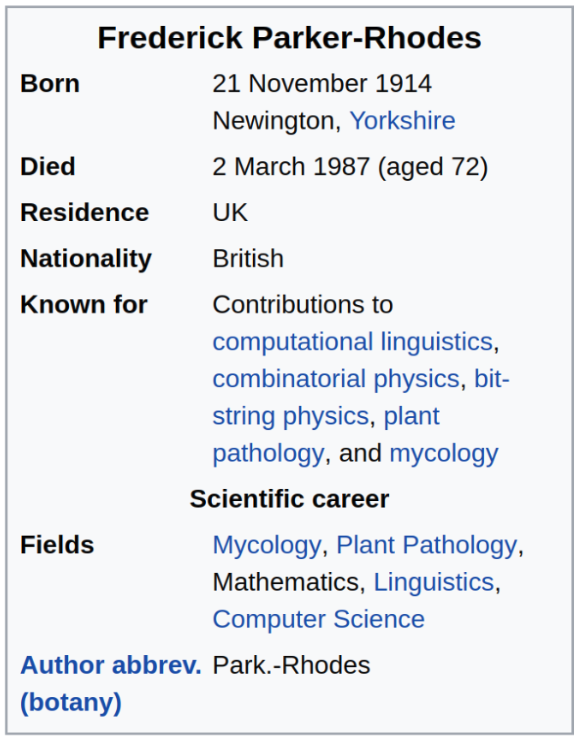
\includegraphics[width=5cm]{wiki}};
      \path[draw, ->] (a) --  (a -|  gal.west) ;


      \node [rounded corners, above =(0.2cm) of a] {{$x$}};

      \visible<2>{
        \node(b) [xshift=4.5cm, yshift=-1cm, rectangle, scale=0.8, draw,thick,fill=blue!0,text width=12em, rounded corners, inner sep =5pt, minimum height=1em]{\baselineskip=50pt \small
          Frederick Parker-Rhodes
(21 November 1914 – 2
March 1987) was an
English linguist, plant
pathologist, computer
scientist, mathematician,
mystic, and mycologist.
          \par};

        \node [rounded corners, above = (0.2cm) of b] {$y_{1:T}$};
        \path[draw, <-] (b) --  (b -| gal.east) ;
      }

      \visible<3>{
        \node(b) [xshift=4.5cm, yshift=-1cm, rectangle, scale=0.8, draw,thick,fill=blue!0,text width=12em, rounded corners, inner sep =5pt, minimum height=1em]{\baselineskip=50pt \small
          Frederick Parker-Rhodes (21 November
1914 – 2 March 1987) was an English
mycology and \alert{plant pathology,
mathematics at the University of UK}.
          \par};

        \node [rounded corners, above = (0.2cm) of b] {$y^*_{1:T}$};
        \path[draw, <-] (b) --  (b -| gal.east) ;
      }



    \end{tikzpicture}
  \end{center}
\end{frame}


\begin{frame}{Alternative Approach: Templated Generation}
  \begin{center}
    \begin{tikzpicture}

      \node (gal) {
\includegraphics[width=1.5cm]{phone}};
      \node [rounded corners, above =(0.2cm) of gal] {$\theta$};


      \node (a) [rectangle, yshift=1cm, xshift=-5cm, scale=0.8, draw,thick,fill=blue!0,text width=13em, rounded corners, inner sep =5pt, minimum height=1em] {
        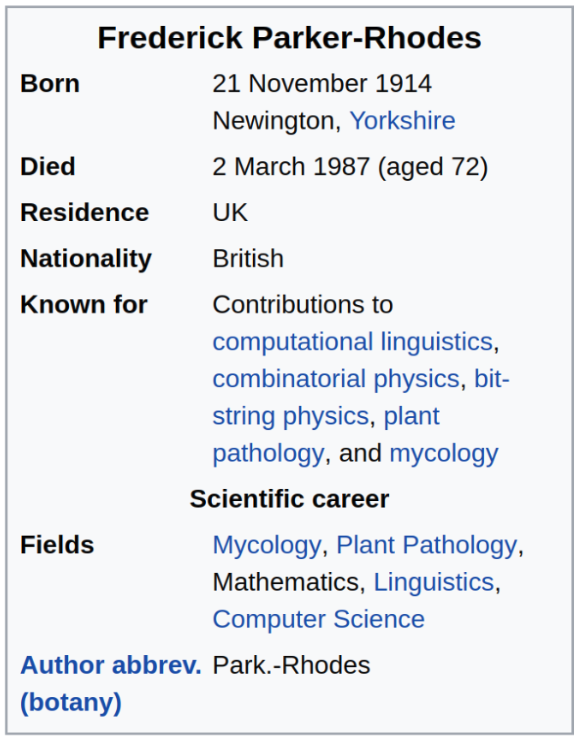
\includegraphics[width=5cm]{wiki}};
      \path[draw, ->] (a) --  (a -|  gal.west) ;


      \node [rounded corners, above =(0.2cm) of a] {{$x$}};

      \visible{
        \node(b) [xshift=4.5cm, yshift=-1cm, rectangle, scale=0.8, draw,thick,fill=blue!0,text width=12em, rounded corners, inner sep =5pt, minimum height=1em]{\baselineskip=50pt \small
          [name] (born [born]) was a
[nationality] [occupation], who
lived in the [residence]. He was
known for contributions to [known\_for].

          \par};

        \node [rounded corners, above = (0.2cm) of b] {$y_{1:T}$};
        \path[draw, <-] (b) --  (b -| gal.east) ;
      }




    \end{tikzpicture}
  \end{center}

\end{frame}


\begin{frame}{Arguments for Rule-Based Generation}
Guarantees about the quality, in particular,
\air


\begin{enumerate}
\item Interpretable in its factual content.
  \air


  \air

\item Controllable in terms of style and form.
  \air



\end{enumerate}

\begin{center}
  Can we achieve this with a deep learning based system?
\end{center}
\end{frame}

\begin{frame}{Learning Neural Templates for Generation}

  \begin{center}
    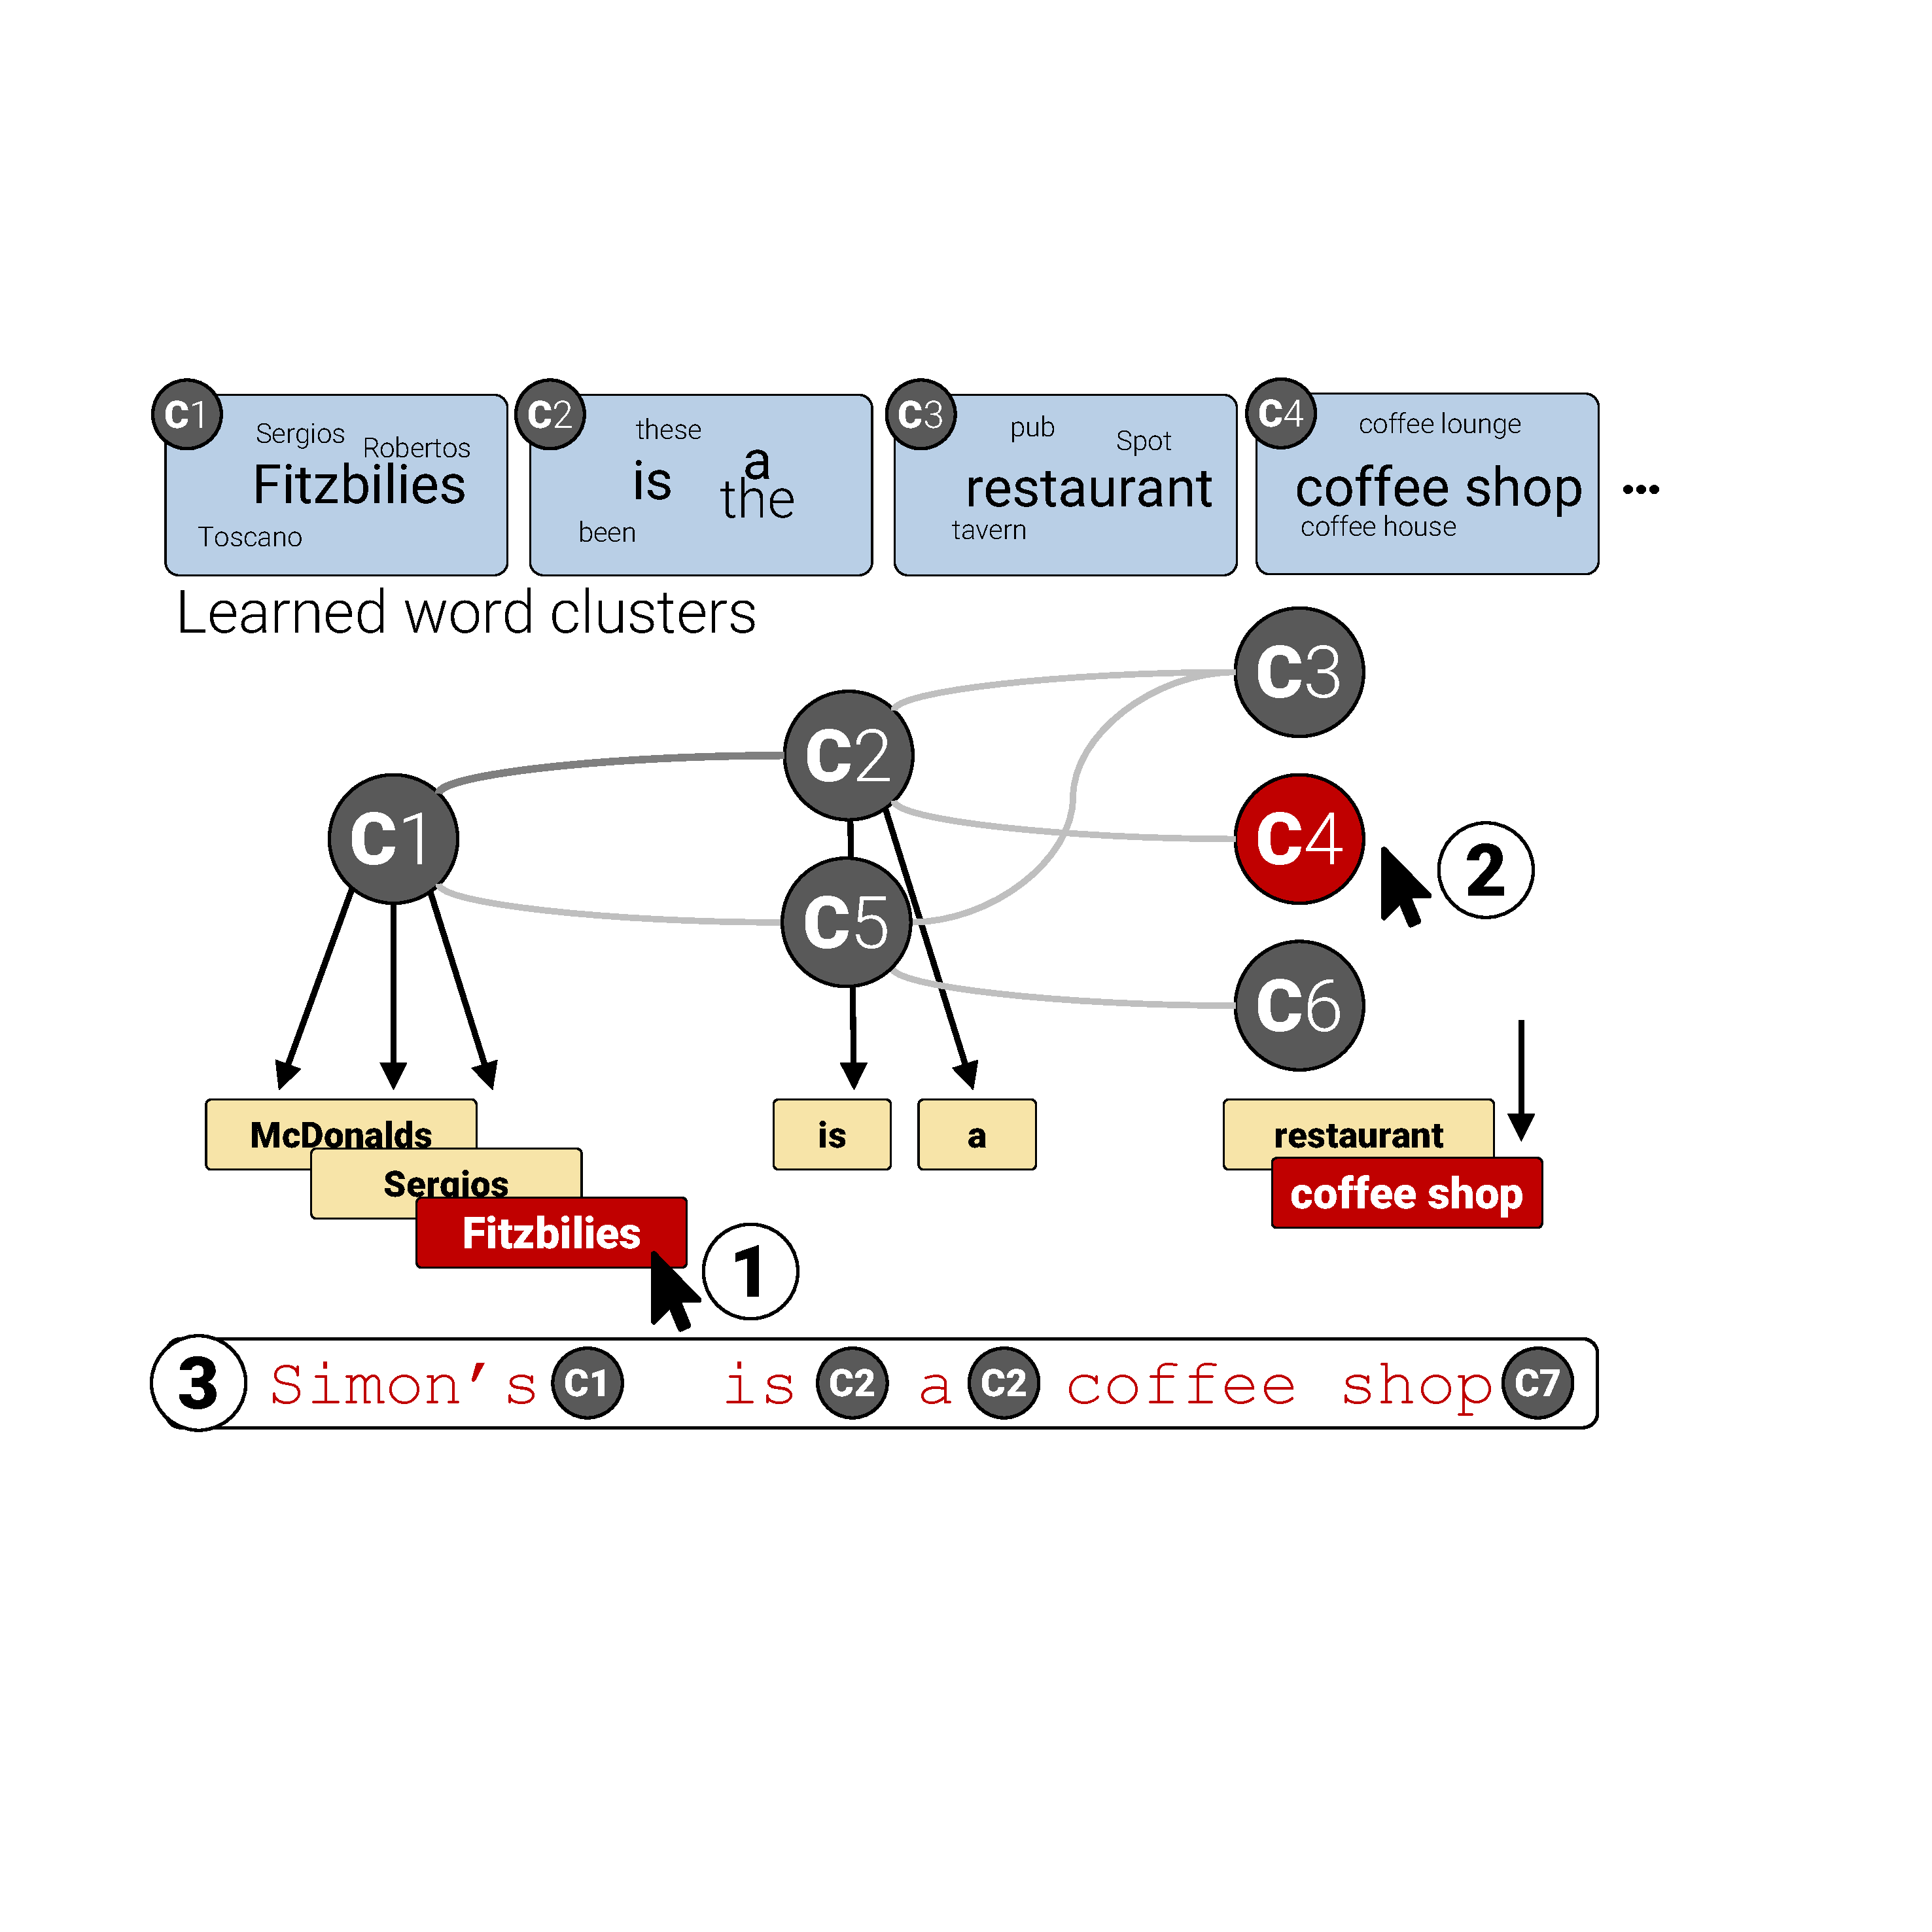
\includegraphics[width=0.7\textwidth]{DecoderVis}
  \end{center}
\end{frame}

\begin{frame}{Approach: Deep Latent-Variable Models}

  Goal: Expose specific choices as \textit{discrete} latent variables $z$.


\begin{align*}
p(y, z\ |\ x \param \theta)
\end{align*}

\begin{itemize}
    \item $x, y, \theta$ as before, \textit{what to talk about / how to say it}
    \item $z$ is a collection of latent variables
\end{itemize}

% \begin{itemize}
%     \item Data consists of $N$ i.i.d samples,
% \end{itemize}

%                 \[ p(x^{(1:N)}, z^{(1:N)} \param \theta ) = \prod_{n=1}^N p(x^{(n)} \given z^{(n)}; \theta) p(z^{(n)};\theta). \]

\end{frame}

\begin{frame}{Example 1: Conditional Sentence Clustering}

Generative process:
\begin{enumerate}
\item Draw cluster $z \in \{1, \ldots, K\}$ from a Categorical.
\item Draw words $y_{1:T}$ from RNN with parameters $\pi_z$.
\end{enumerate}
\[p(y, z| x \param \theta)
       = \mu_{z} \times   \RNN(y_{1:T} \param \pi_z) \]
% \[p(x, z \param \theta)
%       = \mu_{z} \times  \prod_{t=1}^T \softmax(\RNN(\boldh_{t-1}, x_t\param \pi_z))\]
\begin{center}

\begin{tikzpicture}
  %\tikz{
% nodes
\node (dots) {$\ldots$};%
 \node[obs, left=1cm of dots] (x1) {$y_1$};%
 \node[obs, right=1cm of dots] (xT) {$y_T$};%
 \node[latent, above=of dots] (z) {$z$}; %
 \node[const, above=(0.5cm) of z] (mu) {$\mu$};
 \node[const, below left=0.3cm and 0.8cm of x1] (pi) {$\pi$};

% plate
 \plate {plate1} {(dots)(x1)(xT)(z)} {$N$}; %
% edges
 \edge {z} {dots};
 \edge {z} {x1};
 \edge {z} {xT};
 \edge {mu} {z};
 \edge {pi.east} {x1,xT.south};
 \edge {x1} {dots};
 %\edge[bend left] {x1.south} {xT.south};
  \edge {dots} {xT};

 \draw[->]
 (x1) edge[bend right=10] node [right] {} (xT);
 %}
 \end{tikzpicture}
 %}
\end{center}
%\begin{align*}
%\boldh_{z,t} &= \tanh(\mathbf{W}_z \bolde_t +\mathbf{U}_z\boldh_{z,t-1}  + \boldb_{z}) \nonumber \\
%p(x_{t} \given x_{<t} , z) &= \softmax(\mathbf{V} \boldh_{z,t-1} + \boldc)_{x_{t}} \nonumber \\
%p(x_1, \ldots, x_T \given z) &= \prod_{t=1}^{T} p(x_{t} \given x_{<t} , z)
%\end{align*}


\end{frame}


% begin{frame}
% \begin{center}
%     \textbf{ Latent-Variable Model Basics }
%   \end{center}


% \begin{align*}
% p(x, z \param \theta).
% \end{align*}

% \pause
% \begin{itemize}
%     \item $x$ is our observed data
%     \item $z$ is a collection of latent variables
%     \item $\theta$ are the deterministic parameters of the model, such as the neural network parameters
% \end{itemize}

% \pause

% \begin{itemize}
%     \item Data consists of $N$ i.i.d samples,
% \end{itemize}


%                 \[ p(x^{(1:N)}, z^{(1:N)} \param \theta ) = \prod_{n=1}^N p(x^{(n)} \given z^{(n)}; \theta) p(z^{(n)};\theta). \]
% \end{frame}

% \begin{frame}{Posterior Inference}
%     We'll be interested in the \textit{posterior} over latent variables $z$:

%     \begin{align*}
%         p(z \given y, x \param \theta) = \frac{\displaystyle p(y, z | x  \param \theta)}{\displaystyle p(y | x  \param \theta)} = \frac{\displaystyle p(y\given x, z \param  \theta) p(z | x  \param  \theta)}{\displaystyle \sum_{z'} p(y \given x, z'\param  \theta) p(z'| x\param  \theta) }.
%     \end{align*}

%     \air

%     \pause
%     % Why?
%     % \begin{itemize}
%     %   \item Required for training
%     %   \item Latent $z$ gives separation of data.

% % \item Intuition: if I know likely $z^{(n)}$ for $x^{(n)}$, I can learn by maximizing $p(x^{(n)} \given z^{(n)} \param \theta)$.
%         % \begin{itemize}
%         %     \item Intuition: if I know likely $z^{(n)}$ for $x^{(n)}$, I can learn by maximizing $p(x^{(n)} \given z^{(n)} \param \theta)$.
%         % \end{itemize}
%     % \end{itemize}

%     How?

%     \begin{itemize}
%     \item Sum out over all discrete choices (e.g. run $K$ RNNs).
%     \item Variational inference based methods.
%     \end{itemize}

% \end{frame}


\begin{frame}{Example 2: Summary with Copy}
%{(Gu et al, 2016) (Gulcehre et al, 2016)}

Let $z$ be a binary latent variable.
\air
\begin{itemize}
\item If $z = 0$, let the model generate a new word.
\item If $z = 1$, let the model copy a word from the source.
\end{itemize}
\air

% Inference:
\begin{center}
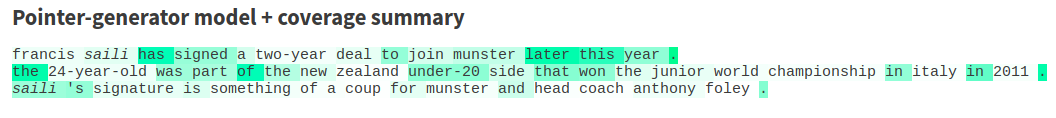
\includegraphics[width=15cm]{seeblog}

% \centerline{\small (See et al, 2017)}
\end{center}
\end{frame}


\begin{frame}{Base Model:  Hidden Semi-Markov Model}

  \air
  \begin{itemize}

  \item HMM: discrete latent states with single emissions  (e.g. words).
    \air

  \item HSMM: discrete latent states produce multiple emissions (e.g. phrases).
    \air

  \item Parameterized with \textit{transition}, \textit{emission},
      and \textit{length} distributions.
      \air

  \end{itemize}

  \begin{figure}
    \centering
    \begin{tikzpicture}[node distance=0.6cm]
    % \draw [step=0.2cm,gray,very thin] (-1.11, -1.11) grid  (1.1, 1.11);
    \node [circle](x){$$} ;
    \node[circle, draw, above right=of x, xshift = 1cm, fill=red!20](z){$z_1$};
    \node[ draw, rounded corners, below=of z, fill=red!10](rnn){};
    \node[circle, draw, below= of rnn](y){$y_1$};
    \node[circle, draw, right= of y](ya){$y_2$};
    \node[circle, draw, right= of ya](yb){$y_3$};
    \node[circle, draw, right= of yb](yc){$y_4$};
    \node[draw, rounded corners,  above= of yc, fill=blue!10](rnnb){};
    \node[circle, draw, above= of rnnb, fill=blue!20](zb){$z_{4}$};
    \draw[-] (z) -- (rnn) -- (y);
    \draw[-]  (rnn) -- (ya);
    \draw[-] (rnn) -- (yb);

    \draw[-] (zb) -- (rnnb) -- (yc);
     \draw (z) --node(mlp)[fill=white, draw, rounded corners]{} (zb);
     % \draw (x.north) edge [bend left=40] (mlp);
     % \draw (x) edge[] (rnn);
     % \draw (x) edge[bend left=20] (rnnb);

    \end{tikzpicture}
  \end{figure}

\end{frame}


\begin{frame}{Our Proposal:  Neural Hidden Semi-Markov Model}

  \begin{itemize}
  \item Employ HSMM as a conditional latent variable language model, $p(y_1, \ldots, y_T, z\ |\ x)$.

    \air
  \item Transition Distribution: NN between states.

    \air
  \item Emission Distribution: Encoder-Decoder, one per state.


  \end{itemize}

  \begin{figure}
    \centering
    \begin{tikzpicture}[node distance=0.6cm]
    \draw [step=0.2cm,gray,very thin] (-1.11, -1.11) grid  (1.1, 1.11);
    \node [draw, circle, fill=black!10](x){$x$} ;
    \node[circle, draw, above right=of x, xshift = 1cm, fill=red!20](z){$z_1$};
    \node[ draw, rounded corners, below=of z, fill=red!10](rnn){Decoder};
    \node[circle, draw, below= of rnn](y){$y_1$};
    \node[circle, draw, right= of y](ya){$y_2$};
    \node[circle, draw, right= of ya](yb){$y_3$};
    \node[circle, draw, right= of yb](yc){$y_4$};
    \node[draw, rounded corners,  above= of yc, fill=blue!10](rnnb){Decoder};
    \node[circle, draw, above= of rnnb, fill=blue!20](zb){$z_{4}$};
    \draw[-] (z) -- (rnn) -- (y);
    \draw[-]  (rnn) -- (ya);
    \draw[-] (rnn) -- (yb);

    \draw[-] (zb) -- (rnnb) -- (yc);
     \draw (z) --node(mlp)[fill=white, draw, rounded corners]{T} (zb);
     \draw (x.north) edge [bend left=40] (mlp);
     \draw (x) edge[] (rnn);
     \draw (x) edge[bend left=20] (rnnb);

    \end{tikzpicture}

    % \caption{HSMM factor graph (under a fixed segmentation) to illustrate parameters. Here we assume $z_1$ is in the ``red'' state (out of $K$ possibilities), and transitions to the ``blue'' state after emitting three words. The transition model, shown as $T$, is a function of the two states and the neural encoded source $x$. The emission model is a function of a ``red'' RNN model (with copy attention over $x$) that generates words 1, 2 and 3. After transitioning, the next word $y_4$ is generated by the ``blue'' RNN, but independently of the previous words.}
    \label{fig:my_label}
  \end{figure}
\end{frame}

\begin{frame}{Technical Methodology:  Fitting Parameters}


  Fit model by minimizing  negative log-marginal likelihood on training data.
    \[ \min_\theta - \log \sum_z p(y, z \ |\ x; \theta)\]
    \air
  Details: Use dynamic programming to efficiently compute HSMM forward algorithm for sum, backprop with autograd, all inference is exact.
    \air
\end{frame}


\begin{frame}{From Neural HSMM to Templates}
  \begin{figure}
    \centering
    \begin{tikzpicture}[node distance=0.6cm]
    \draw [step=0.2cm,gray,very thin] (-1.11, -1.11) grid  (1.1, 1.11);
    \node [draw, circle, fill=black!10](x){$x$} ;
    \node[circle, draw, above right=of x, xshift = 1cm, fill=red!20](z){$z_1$};
    \node[ draw, rounded corners, below=of z, fill=red!10](rnn){Decoder};
    \node[circle, draw, below= of rnn](y){$y_1$};
    \node[circle, draw, right= of y](ya){$y_2$};
    \node[circle, draw, right= of ya](yb){$y_3$};
    \node[circle, draw, right= of yb](yc){$y_4$};
    \node[draw, rounded corners,  above= of yc, fill=blue!10](rnnb){Decoder};
    \node[circle, draw, above= of rnnb, fill=blue!20](zb){$z_{4}$};
    \draw[-] (z) -- (rnn) -- (y);
    \draw[-]  (rnn) -- (ya);
    \draw[-] (rnn) -- (yb);

    \draw[-] (zb) -- (rnnb) -- (yc);
     \draw (z) --node(mlp)[fill=white, draw, rounded corners]{T} (zb);
     \draw (x.north) edge [bend left=40] (mlp);
     \draw (x) edge[] (rnn);
     \draw (x) edge[bend left=20] (rnnb);

    \end{tikzpicture}

    % \caption{HSMM factor graph (under a fixed segmentation) to illustrate parameters. Here we assume $z_1$ is in the ``red'' state (out of $K$ possibilities), and transitions to the ``blue'' state after emitting three words. The transition model, shown as $T$, is a function of the two states and the neural encoded source $x$. The emission model is a function of a ``red'' RNN model (with copy attention over $x$) that generates words 1, 2 and 3. After transitioning, the next word $y_4$ is generated by the ``blue'' RNN, but independently of the previous words.}
    \label{fig:my_label}
  \end{figure}


    Compute argmax latent variables to find common \textit{templates}.
    \[ z_{1:T}^* = \argmax_{z_{1:T}} p(y_{1:T}, z_{1:T} \ |\ x; \theta)\]


    {\it
    [The Wrestlers]$_{185}$ [is a]$_{29}$ [coffee shop]$_{164}$ [that serves]$_{188}$ [English]$_{139}$ [food]$_{18}$ [in the]$_{32}$ [moderate]$_{125}$ [price range]$_{180}$ [.]$_{90}$
  }
\end{frame}


\begin{frame}{Example Templates: Wikipedia}
  \begin{center}
    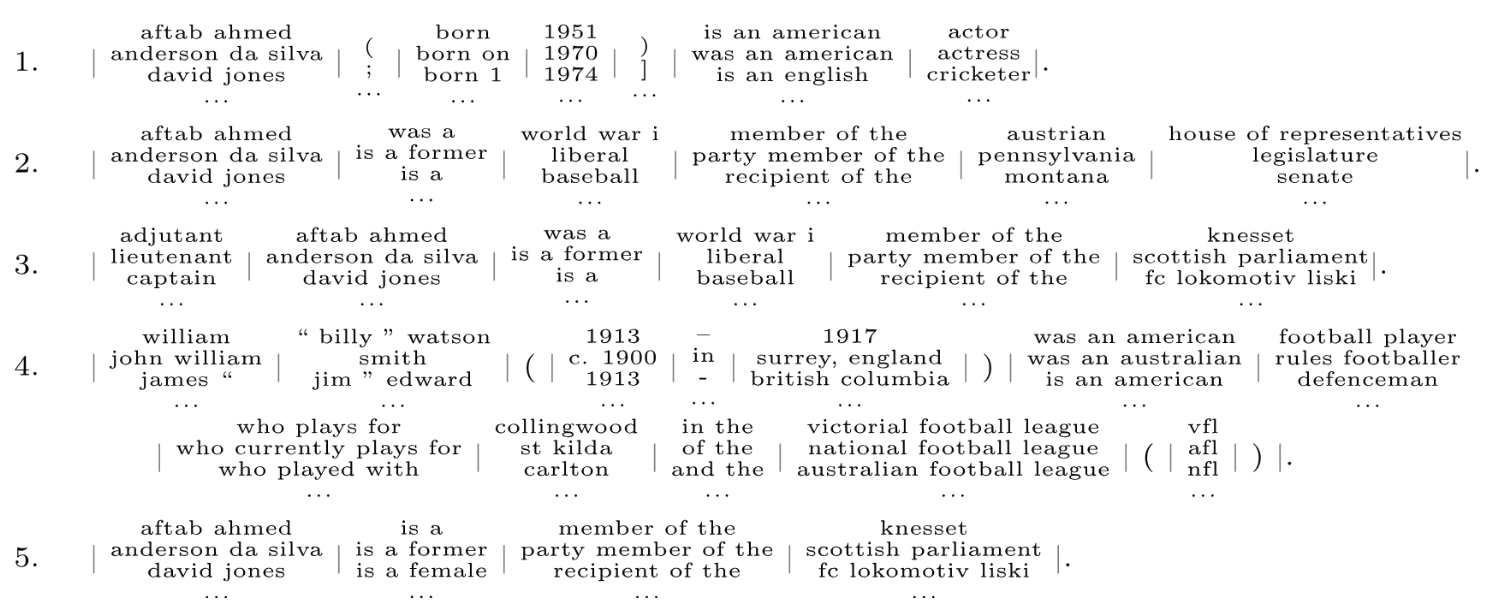
\includegraphics[width=0.9\textwidth]{extemp}
  \end{center}
\end{frame}

% \begin{frame}{ Latent Variable Models for Generation}
%   \textbf{Ongoing Work:} Can we develop other discrete latent-variable models for generation?

%   \air

%   \textbf{Goals:}

%     \begin{itemize}
%     \item Model Control
%     \item Model Debugging
%     \item Model Uncertainty
%     \end{itemize}
% \end{frame}




% \begin{frame}
%   \begin{figure}
%     \centering

%     \footnotesize
% \begin{tabular}{@{}ll@{}}
% \toprule
% \bf Meaning Representation        & \begin{tabular}[c]{@{}l@{}}name{[}The Golden Palace{]},  eatType{[}coffee shop{]},  food{[}Fast food{]}, \\ priceRange{[}cheap{]},  customer rating{[}5 out of 5{]},  area{[}riverside{]}\end{tabular}         \\ \midrule
% \bf Reference & \begin{tabular}[c]{@{}l@{}}A coffee shop located on the riverside  called The Golden Palace,  \\ has a 5 out of 5 customer rating.  Its price range are fairly cheap  \\for its excellent Fast food.\end{tabular} \\ \bottomrule
% \end{tabular}
%   \end{figure}

% \end{frame}

% \begin{frame}{Standard Approach}


% \textbf{Step 1: Encode the Source}
% \air

% \begin{small}
% Fitzbillies,type[coffee shop],price[$<$ \pounds 20],food[Chinese],rate[3/5],area[city centre]
% \end{small}

% \vspace{0.3cm}

% \textbf{Step 2: Generate with RNN Decoder}

% \air

% \underline{Fitzbillies}  is a  \underline{coffee shop}  providing  \underline{Chinese} food in the  moderate  price range  .  It is  located in the  \underline{city centre}  .  Its customer rating is  \underline{3} out of \underline{5}.

% \end{frame}

% \begin{frame}{Issues}
% \begin{enumerate}
% \item Interpretable in its content selection?
%   \air

%   \textit{Decisions may come from anywhere in the source $x$.}

%   \air

% \item Controllable in terms of style and form?
%   \air

%   \textit{Rely on a learned system to determine content.}
% \end{enumerate}

%\end{frame}

\begin{frame}{Neural Template Generation Approach}
  \vspace{-1cm}
  \begin{center}
    \begin{tikzpicture}

      \node (gal) {
\includegraphics[width=1.5cm]{phone}};
      \node [rounded corners, above =(0.2cm) of gal] {$\theta$ (HSMM)};
      \node (a) [rectangle, yshift=1cm, xshift=-5cm, scale=0.7, draw,thick,fill=blue!0,text width=11em, rounded corners, inner sep =5pt, minimum height=1em] {
        \small
        \begin{tabular}[]{lc}
          \textbf{Fitzbillies} & \\
          \toprule
          type & [coffee shop] \\
          price & $<$ \pounds 20 \\
          food & Chinese \\
          rating  & 3/5 \\
          area & city centre] \\
          \bottomrule
        \end{tabular}};



      % \path<2>[draw, ->] (a) --  (a -|  gal.west) ;


      \node [rounded corners, above =(0.2cm) of a] {\alert<1>{$x$}};
      \path[draw, ->] (a) --  (gal.west);
      \visible<2->{
        \node(b) [xshift=-5cm, yshift=-2.5cm, rectangle, scale=0.7, draw,thick,fill=blue!0,text width=18em, rounded corners, inner sep =5pt, minimum height=1em]{\baselineskip=50pt \small
$\textcolor{gray}{|} $ $ \substack{\text{The \rule{15pt}{1pt}}\\\text{\rule{15pt}{1pt}}\\ \dots}
\ \textcolor{gray}{|} \  $ $ \substack{\text{is a}\\\text{is an}\\\text{is an expensive}\\ \dots}
\ \textcolor{gray}{|} \  $ $ \text{\rule{15pt}{1pt}} \ \textcolor{gray}{|} \  $ $ \substack{\text{providing}\\\text{serving}\\\text{offering}\\ \dots}
\ \textcolor{gray}{|} \  $ $ \text{\rule{15pt}{1pt}} \ \textcolor{gray}{|} \  $ $ \substack{\text{food}\\\text{cuisine}\\\text{foods}\\ \dots}
\ \textcolor{gray}{|} \  $ $ \text{in the} \ \textcolor{gray}{|} \  $ $ \substack{\text{high}\\\text{moderate}\\\text{less than average}\\ \dots}
\ \textcolor{gray}{|} \  $ $ \substack{\text{price}\\\text{price range}\\ \dots}
\ \textcolor{gray}{|} \  $ $ \text{.}$ $\textcolor{gray}{|}$ $ \text{It is} \ \textcolor{gray}{|} \  $ $ \substack{\text{located in the}\\\text{located near}\\\text{near}\\ \dots}
\ \textcolor{gray}{|} \  $ $ \text{\rule{15pt}{1pt}} \ \textcolor{gray}{|} \  $ $ \text{.}$ $ \textcolor{gray}{|} \  $ $ \substack{\text{Its customer rating is}\\\text{Their customer rating is}\\\text{Customers have rated it}\\ \dots}
\ \textcolor{gray}{|} \  $ $ \text{\rule{15pt}{1pt} out of \rule{15pt}{1pt}} \ \textcolor{gray}{|} \  .$
          \par};

        \node [rounded corners, above = (0.1cm) of b] {$z_{1:T}$};
        \path[draw, ->] (b) --  (gal.west);
      }

      \visible<3->{
        \node(c) [xshift=4.5cm, rectangle, scale=0.75, draw,thick,fill=blue!0,text width=20em, rounded corners, inner sep =5pt, minimum height=1em] {\baselineskip=50pt \small $\|$  \underline{Fitzbillies} $\|$   is a $\|$    \underline{coffee shop} $\|$   providing $\|$  \underline{Chinese} $\|$ food $\|$ in the $\|$  moderate $\|$ price range $\|$ . $\|$ It is  $\|$ located in the $\|$ \underline{city centre} $\|$ . $\|$ Its customer rating is $\|$ \underline{3} out of \underline{5} $\|$ . \par };
      \node [rounded corners, above = (0.1cm) of c] { $y_{1:T}$};
      \path[draw, ->] (gal.east) -- (c);
    }


    \end{tikzpicture}
  \end{center}
\end{frame}

% \textbf{Step 1: Encode the Source}

% \begin{small}
% Fitzbillies,ty[coffee shop],pr[$<$ \pounds 20],food[Chinese],cust[3/5],area[city centre]
% \end{small}

% \pause
% \air
% \textbf{Step 2: Select a \textit{Template}}

%     \begin{center}

% $\textcolor{gray}{|} $ $ \substack{\text{The \rule{15pt}{1pt}}\\\text{\rule{15pt}{1pt}}\\ \dots}
% \ \textcolor{gray}{|} \  $ $ \substack{\text{is a}\\\text{is an}\\\text{is an expensive}\\ \dots}
% \ \textcolor{gray}{|} \  $ $ \text{\rule{15pt}{1pt}} \ \textcolor{gray}{|} \  $ $ \substack{\text{providing}\\\text{serving}\\\text{offering}\\ \dots}
% \ \textcolor{gray}{|} \  $ $ \text{\rule{15pt}{1pt}} \ \textcolor{gray}{|} \  $ $ \substack{\text{food}\\\text{cuisine}\\\text{foods}\\ \dots}
% \ \textcolor{gray}{|} \  $ $ \text{in the} \ \textcolor{gray}{|} \  $ $ \substack{\text{high}\\\text{moderate}\\\text{less than average}\\ \dots}
% \ \textcolor{gray}{|} \  $ $ \substack{\text{price}\\\text{price range}\\ \dots}
% \ \textcolor{gray}{|} \  $ $ \text{.}$ $\textcolor{gray}{|}$ $ \text{It is} \ \textcolor{gray}{|} \  $ $ \substack{\text{located in the}\\\text{located near}\\\text{near}\\ \dots}
% \ \textcolor{gray}{|} \  $ $ \text{\rule{15pt}{1pt}} \ \textcolor{gray}{|} \  $ $ \text{.}$ $ \textcolor{gray}{|} \  $ $ \substack{\text{Its customer rating is}\\\text{Their customer rating is}\\\text{Customers have rated it}\\ \dots}
% \ \textcolor{gray}{|} \  $ $ \text{\rule{15pt}{1pt} out of \rule{15pt}{1pt}} \ \textcolor{gray}{|} \  .$
%     \end{center}
% \pause
% \air
% \textbf{Step 3: Fill-in Each Segment}
%     \air


% $\|$ \underline{Fitzbillies} $\|$  \pause is a $\|$ \pause   \underline{coffee shop} $\|$ \pause  providing $\|$  \underline{Chinese} $\|$ food $\|$ in the $\|$  moderate $\|$ price range $\|$ . $\|$ It is  $\|$ located in the $\|$ \underline{city centre} $\|$ . $\|$


    % \caption{An example from the E2E Generation dataset~\citep{novikova2017e2e}; knowledge base $x$ (top) contains 5 records, and $\hat{y}$ (middle) is a system generation; records are shown as \texttt{type[value]}.
    % (bottom) An induced neural template learned by the system and employed in generating $\hat{y}$. %Each cell shows the possible output choices and each underscore represents a slot fillable with copy attention.
    % Each cell represents a segment in the learned segmentation, and underscores show where slots are (typically) filled through copy attention during generation.
    % }

% \end{frame}


% \begin{frame}{Criteria}

% \begin{enumerate}
% \item Interpretable in its content selection.
%   \air

%   \textit{Decisions are localized to a segment of the template.}

%   \air

% \item Easily controllable in terms of style and form.
%   \air

%   \textit{Alternative realizations through different templates.}
% \end{enumerate}


% \air

% \pause



% \alert{However:} templates feel much less ``end-to-end''.
% How can we learn them from data?

% \end{frame}



% \begin{frame}{Neural Template}
% \air

%       \begin{center}

% $\textcolor{gray}{|} $ $ \substack{\text{The \rule{15pt}{1pt}}\\\text{\rule{15pt}{1pt}}\\ \dots}
% \ \textcolor{gray}{|} \  $ $ \substack{\text{is a}\\\text{is an}\\\text{is an expensive}\\ \dots}
% \ \textcolor{gray}{|} \  $ $ \text{\rule{15pt}{1pt}} \ \textcolor{gray}{|} \  $ $ \substack{\text{providing}\\\text{serving}\\\text{offering}\\ \dots}
% \ \textcolor{gray}{|} \  $ $ \text{\rule{15pt}{1pt}} \ \textcolor{gray}{|} \  $ $ \substack{\text{food}\\\text{cuisine}\\\text{foods}\\ \dots}
% \ \textcolor{gray}{|} \  $ $ \text{in the} \ \textcolor{gray}{|} \  $ $ \substack{\text{high}\\\text{moderate}\\\text{less than average}\\ \dots}
% \ \textcolor{gray}{|} \  $ $ \substack{\text{price}\\\text{price range}\\ \dots}
% \ \textcolor{gray}{|} \  $ $ \text{.}$ $\textcolor{gray}{|}$ $ \text{It is} \ \textcolor{gray}{|} \  $ $ \substack{\text{located in the}\\\text{located near}\\\text{near}\\ \dots}
% \ \textcolor{gray}{|} \  $ $ \text{\rule{15pt}{1pt}} \ \textcolor{gray}{|} \  $ $ \text{.}$ $ \textcolor{gray}{|} \  $ $ \substack{\text{Its customer rating is}\\\text{Their customer rating is}\\\text{Customers have rated it}\\ \dots}
% \ \textcolor{gray}{|} \  $ $ \text{\rule{15pt}{1pt} out of \rule{15pt}{1pt}} \ \textcolor{gray}{|} \  .$
%     \end{center}
% \end{frame}

% \begin{frame}{Experimental Setup}

%   \begin{itemize}
%   \item Two datasets, E2E challenge and WikiBio
%     \air
%   \item Training with 35 and 65 state models, each 1x300 LSTMs.
%     \air
%   \item Extract 100 most common templates for each.
%     \air
%   \item Vocabulary limited to non-copy-able words.
%     \air

%   \item Generation with beam search with a pre-selected template.
%   \end{itemize}
% \end{frame}




% \begin{frame}{WikiBio (500k)}

%   \begin{center}



%       \begin{figure}[t]
% \centering
% \begin{tabular}{@{}l@{}}
% \toprule
% \\
% % \begin{tabular}[c]{c}
% %   \hspace{2.5cm}
% %     % \includegraphics[scale=0.7]{wbpage_cropped.pdf}
% % \end{tabular}
% \midrule
% \begin{tabular}[c]{@{}l@{}}
% {\small Frederick Parker-Rhodes (21 March 1914 - 21 November} \\
% {\small 1987) was an English linguist, plant pathologist, computer} \\
% {\small scientist, mathematician, mystic, and mycologist.}
% \end{tabular} \\
% \bottomrule
% \end{tabular}
% % \caption{An example from the WikiBio dataset~\citep{lebret2016neural} for entity \texttt{Frederick Parker-Rhodes}; $x$ (top) and $y$ (bottom) is the corresponding reference generation.}
% \label{fig:wbex}
% \end{figure}

%   \end{center}
% \end{frame}






% \begin{frame}{WikiBio}
% \begin{table}[t!]
% \small
% \centering
% \begin{tabular}{@{}lccc@{}}
% \toprule
%  & BLEU & NIST & ROUGE-4\\
% \midrule
% Conditional KN-LM  & 19.8 & 5.19 & 10.7 \\
% NNLM (field)  & 33.4 & 7.52 & 23.9 \\
% NNLM (field \& word)  & 34.7 & 7.98 & 25.8 \\
% Neural Template &  33.8 & 7.51 & 28.2 \\
% \bottomrule
% \end{tabular}
% \label{tab:wb}
% \end{table}

% \begin{itemize}
% \item Custom KN and NNLM Baselines from LeBret et al (2016)
% \end{itemize}k

% \end{frame}



% \begin{frame}
% \end{frame}

\begin{frame}[fragile]{Issue 1: Interpretability}

  \begin{center}



  \begin{table}[t]
\small
\centering

\begin{tabular}{@{}l@{}}
  \toprule
  \textbf{kenny warren} \\
  \midrule
  \begin{tabular}[c]{@{}l@{}}
    \textbf{name:} kenny warren, \textbf{birth date:} 1 april 1946, \\
    \textbf{birth name:} kenneth warren deutscher, \textbf{birth place:} brooklyn, new york, \\ \textbf{occupation:} ventriloquist, comedian, author, \\
    \textbf{notable work:} book - the revival of ventriloquism in america \\
  \end{tabular}         \\
  \midrule

  \begin{tabular}[c]{@{}l@{}}
    1. \colorbox{green}{kenny warren deutscher} (\colorbox{pink}{april 1, 1946}) is an \colorbox{cyan}{american} ventriloquist. \\
    2. \colorbox{green}{kenny warren deutscher} (\colorbox{pink}{april 1, 1946}, brooklyn,) is an \colorbox{cyan}{american} ventriloquist.\\
    3. \colorbox{green}{kenny warren deutscher} (\colorbox{pink}{april 1, 1946}) is an \colorbox{cyan}{american} \\
    \hspace{1cm} ventriloquist, best known for his the revival of ventriloquism. \\
    4. \colorbox{yellow}{``kenny'' warren} is an \colorbox{cyan}{american} ventriloquist. \\
5. kenneth warren \colorbox{yellow}{``kenny'' warren} (born \colorbox{pink}{april 1, 1946}) is \\
\hspace{1cm} an \colorbox{cyan}{american} ventriloquist, and author. \\
\end{tabular} \\
\bottomrule
\end{tabular}
\label{tab:wbcontrol}
\end{table}

  \end{center}
\end{frame}


\begin{frame}{Issue 2: Controllability}

  \begin{table}[t]
\small
\centering
\begin{tabular}{@{}l@{}}
\toprule
\textbf{The Golden Palace} \\
\midrule
\begin{tabular}[c]{@{}l@{}}
name[The Golden Palace], type[coffee shop], food[Chinese], \\
priceRange[cheap] custRating[5 out of 5], area[city centre], \\
\end{tabular}         \\
\midrule
\begin{tabular}[c]{@{}l@{}}
1. The Golden Palace is a coffee shop located in the city centre. \\
2. In the city centre is a cheap Chinese coffee shop called \\
\; \; The Golden Palace. \\
3. The Golden Palace that serves Chinese food in the cheap \\
\; \; price range. It is located in the city centre.  Its customer \\
\; \; rating is 5 out of 5. \\
4. The Golden Palace is a Chinese coffee shop. \\
5. The Golden Palace is a Chinese coffee shop \\
\; \; with a customer rating of 5 out of 5. \\
\end{tabular} \\
\bottomrule
\end{tabular}
% \caption{Impact of varying the template $z^{(i)}$ for a single $x$ from the E2E dataset.}
\label{tab:e2econtrol}
\end{table}
\end{frame}


\begin{frame}{Results}
\begin{table}[t!]
\small
\centering
\begin{tabular}{@{}lccc@{\hspace{2.5mm}}c@{\hspace{2.5mm}}c@{}}
\toprule
 & BLEU & NIST \\
\midrule
% Val & & &  \\
% \midrule

% Substitution  & 43.71 & 6.72 \\
% Neural Template & 66.06 & 7.93 \\
% Full Neural Model & 69.25 & 8.48 \\
% \midrule
Test  & & \\
\midrule

Substitution & 43.78 & 6.88 \\
Neural Template    & 56.72 & 7.63 \\
Full Neural Model & 65.93 & 8.59 \\
\bottomrule
\end{tabular}
\begin{table}[t!]
\small
\centering
\begin{tabular}{@{}lccc@{}}
\toprule
 & BLEU & NIST & ROUGE-4\\
\midrule
Conditional KN-LM  & 19.8 & 5.19 & 10.7 \\
NNLM (field)  & 33.4 & 7.52 & 23.9 \\
NNLM (field \& word)  & 34.7 & 7.98 & 25.8 \\
Neural Template &  33.8 & 7.51 & 28.2 \\
\bottomrule
\end{tabular}
\label{tab:wb}
\end{table}

% \caption{Comparison of the system of \citet{duvsek2016sequence}, which forms the baseline for the E2E challenge, a non-parametric, substitution-based baseline (see text), and our HSMM model on the validation and test portions of the E2E dataset. ``ROUGE'' is ROUGE-L. Models are evaluated using the official E2E NLG Challenge scoring scripts.}
\label{tab:e2e}
\end{table}

\end{frame}

\begin{frame}{Talk Outline}

  \begin{enumerate}
  \item Background: Core Model and Implementation
    \air
  \item Work 1: Rethinking Model Training (\textit{Beam Search Optimization})
    \air

  \item Work 2: Rethinking  Generation  (\textit{Learning Neural Templates})
    \air

  \item \textbf{Future Challenges in Text Generation}
  \end{enumerate}
\end{frame}


\begin{frame}{Three Challenge in Text Generation}
  \begin{enumerate}
  \item Long-Form Generation with High-Level Reasoning
    \air
  \item Compact and Efficient Generation
    \air
  \item Latent-Variable Modeling for NLP
  \end{enumerate}
\end{frame}

% \begin{frame}{Future Work}

%   \begin{center}
%   \begin{tikzpicture}
%     \node[rounded corners, draw] (ana) at (-15mm, 15mm) {Analysis};
%     \node[rounded corners, draw] (meth) at (0mm, 30mm) {\ Methods\phantom{p}};
%     \node[rounded corners, draw] (app) at (25mm, 30mm) {Applications};
%     \node[rounded corners, draw] (und) at (35mm, 15mm) {Understanding};
%     \node[rounded corners, draw] (dep) at (25mm, 0mm){Deployment};
%     \node[rounded corners, draw] (imp) at (0, 0) {Implement};
%     \draw (ana) -- (meth) --(app) -- (und) -- (dep) -- (imp) -- (ana);
%   \end{tikzpicture}
%   \end{center}
% \end{frame}


\begin{frame}{Long-Form Generation with Explicit Reasoning}
  \begin{center}
    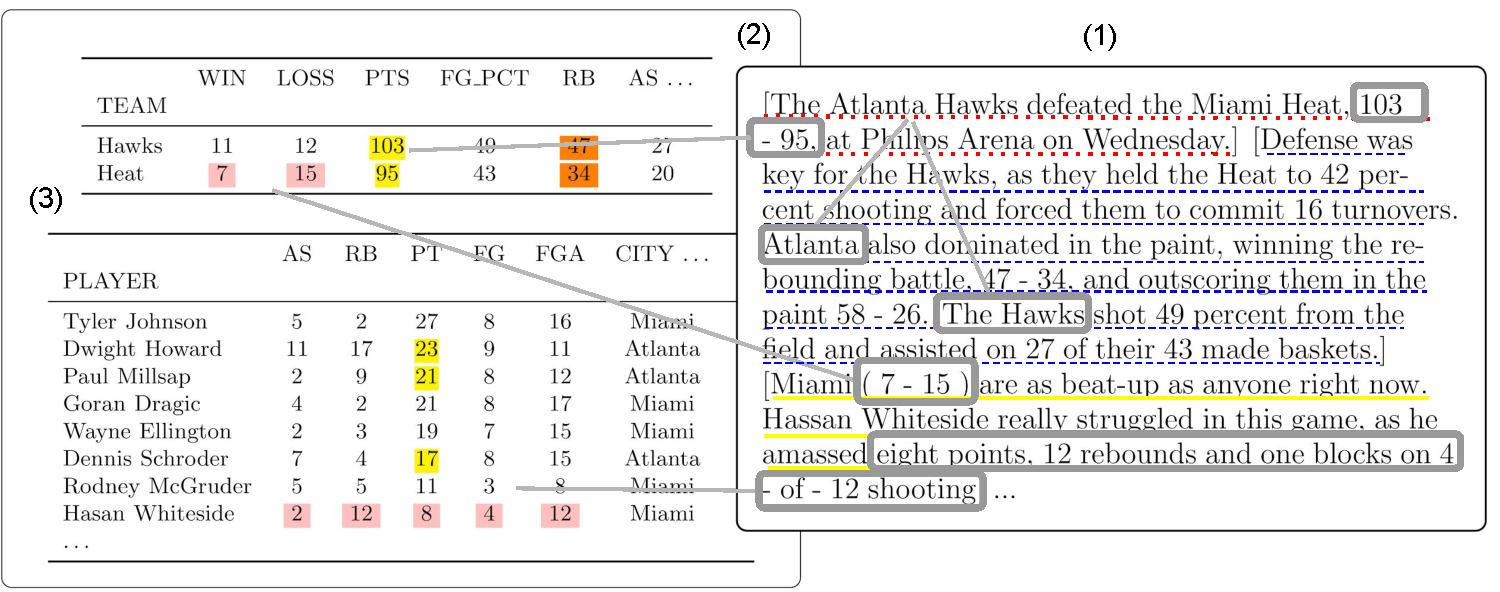
\includegraphics[width=0.85\linewidth]{basketball}
  \end{center}
\end{frame}


\begin{frame}{Summary}
  \begin{center}
    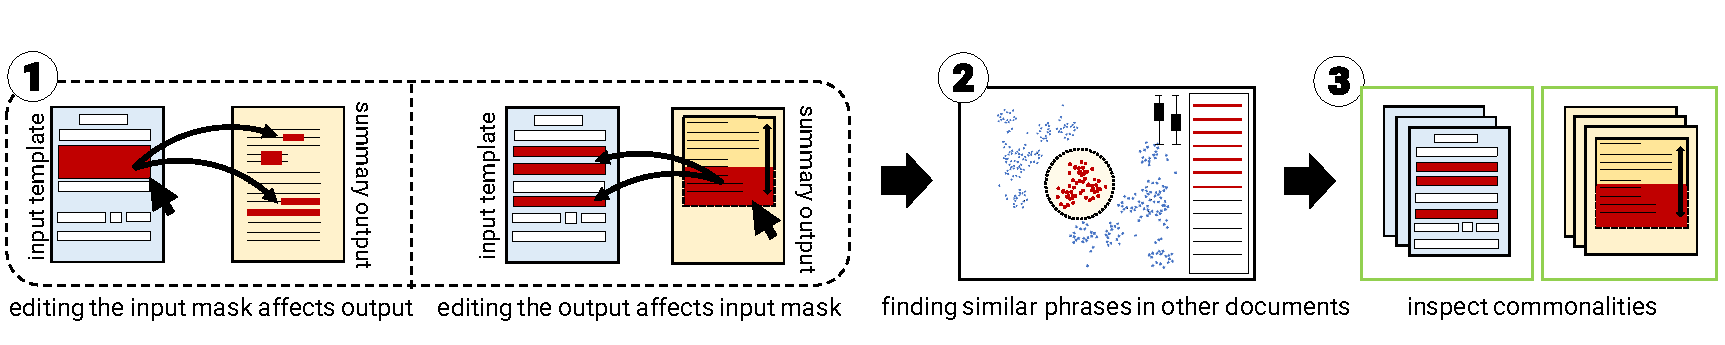
\includegraphics[width=\textwidth]{summary}
  \end{center}
\end{frame}

\begin{frame}{Hardware for NLP}
\research{Preprint}
\begin{center}
  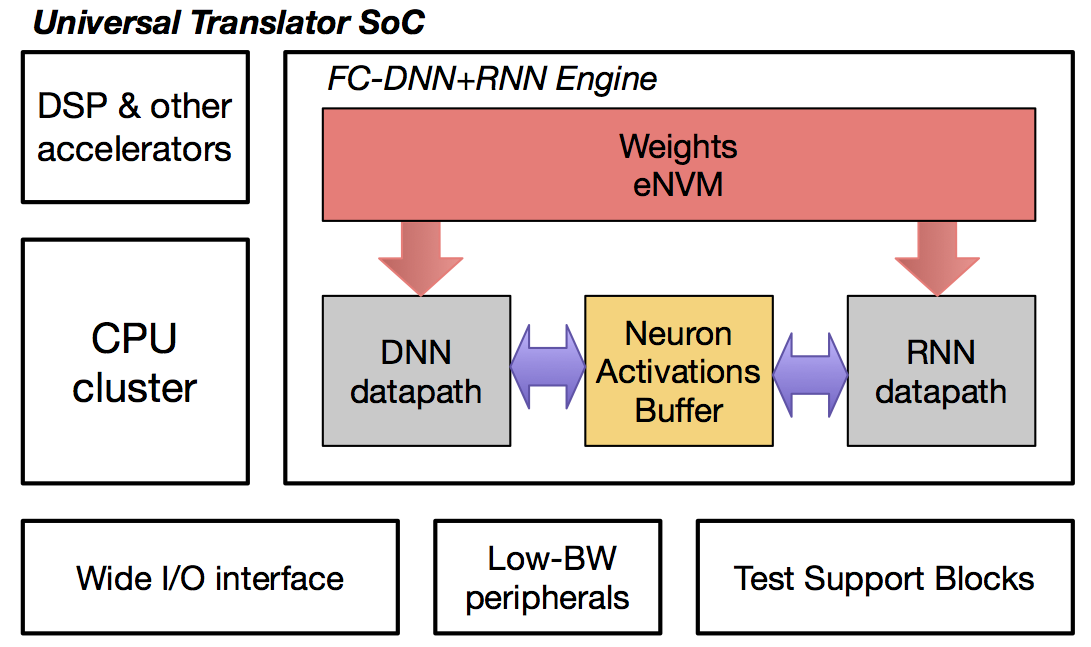
\includegraphics[height=0.8\textheight]{testchip}
\end{center}
\end{frame}


\begin{frame}{Latent-Variable Modeling for NLP}
\research{Preprint}

\begin{center}

\includegraphics[width=2.5cm]{pyro}

\air

  \begin{tikzpicture}
\node[latent] (Y) {$y$};
\node[factor, xshift=1.25cm] (FYS) {$F$};
\node[latent, xshift=2.5cm](S) {$z$};
\node[factor, xshift=3.75cm](FS) {$G$};
\node[xshift=1.25cm, yshift=-0.5cm]() {$T$};
\node[obs, xshift=5cm](X) {$\mathbf{x}$};
\node[obs, xshift=2.5cm, yshift=1.3cm] (A) {$a$};
\node[obs, xshift=2.5cm, yshift=-1.45cm] (L) {$l$};


\plate [inner sep=0.1cm, xshift=0cm, yshift=0.0cm] {t} {(FS)(S)(FYS)} {};
\plate [inner xsep= 0.3cm, inner ysep= 0.2cm, xshift=-0.1cm, yshift=-0.1cm] {a} {(Y)(FYS)(S)(A)(FS)} {};
\plate [inner xsep= 0.3cm, inner ysep= 0.1cm, xshift=0.1cm, yshift=0.2cm] {l} {(Y)(FYS)(S)(L)(FS)} {};
\node[caption, below left=-0.1cm and -0.3cm of a-wrap.north west] {$|\cal{A}|$};
\node[caption, below left=-0.5cm and -0.4cm of l-wrap.south east] {$|\cal{L}|$};

\draw (Y) -- (FYS);
\draw (X) -- (FS);
\draw[-] (X) to [bend left=25] (FYS);
\draw (FYS) -- (S);
\draw (S) -- (FS);
\draw (FS) -- (A);
\draw (FS) -- (L);
\draw[-] (FYS) to [] (A);
\draw[-] (FYS) to [] (L);
\end{tikzpicture}
\end{center}
\end{frame}

% \begin{frame}{Learning Neural Reasoning-Based Models}
%   \begin{center}
%     \movie[width=\textwidth, repeat, height=0.85\textheight, width=\textwidth, poster, showcontrols]{Temporary}{videos/latnm.mp4}
%   \end{center}
% \end{frame}


\begin{frame}
  Thanks
\end{frame}



\begin{frame}

\end{frame}